\chapter{Zuren, basen en pH}\label{ch:g9:acids-bases-ph}

Op een plank in de keuken staan een citroen, een fles azijn, een stuk
zeep en een doos baksoda; onder de gootsteen een fles ontstopper met een
zwart-rood waarschuwingsetiket. Sommige hiervan smaken zuur, sommige
voelen glibberig aan, sommige kunnen de huid verbranden. Eén enkele
schaal, genummerd van 0 tot 14, deelt ze allemaal in --- en dezelfde
schaal wordt gebruikt voor zwembaden, tuingrond, het bloed en de
oceanen.

\begin{recall}
\omterm{def:g9:ions:ion}{Ionen} zijn \omterm{def:g7:atoms-and-molecules:atom}{atomen} of groepen \omterm{def:g7:atoms-and-molecules:atom}{atomen} die een lading dragen; een \omterm{def:g9:ions:ion}{kation}
zoals \ce{Na+} is positief, een \omterm{def:g9:ions:ion}{anion} zoals \ce{Cl-} of \ce{OH-}
negatief. Ionenoplossingen bevatten \omterm{def:g9:ions:ion}{ionen} met de aanduiding (aq), die
vrij bewegen (\cref{ch:g9:ions}).
\end{recall}

\begin{omfigure}
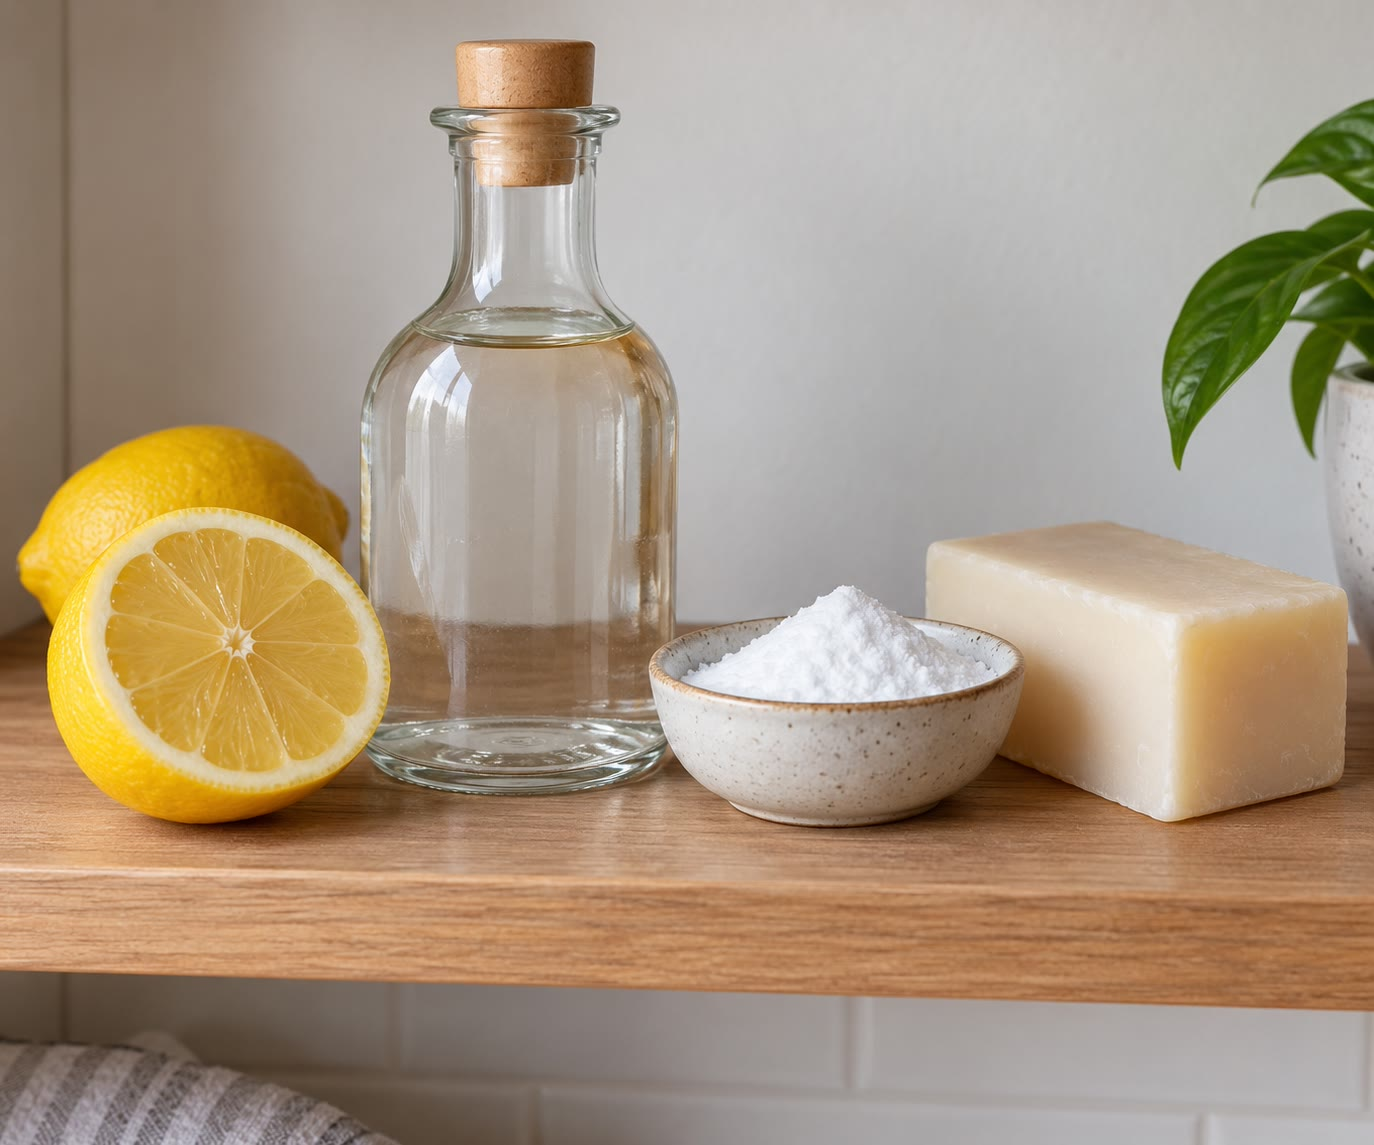
\includegraphics[width=0.55\linewidth]{images/book1/ai/g9-kitchen-shelf.jpg}

{\small Citroen, azijn, zeep en baksoda: zuren en basen in de keuken.}
\end{omfigure}

\section{Zure, basische en neutrale oplossingen}

\begin{definition}[Zure, basische en neutrale oplossingen]\label{def:g9:acids-bases-ph:acidic}
Elke \omterm{def:g6:solutions-and-solubility:solute}{waterige oplossing} bevat waterstofionen \ce{H+(aq)} en
\omterm{def:g9:ions:ion}{hydroxide-ionen} \ce{OH-(aq)}. Een oplossing is een \emph{zure
oplossing}\index{zure oplossing} als ze meer \ce{H+}-ionen dan
\ce{OH-}-ionen bevat, een \emph{basische oplossing}\index{basische oplossing}
als ze meer \ce{OH-}-ionen dan \ce{H+}-ionen bevat, en een
\emph{neutrale oplossing}\index{neutrale oplossing} als ze van allebei
evenveel bevat.
\end{definition}

\begin{example}[Drie oplossingen]\label{ex:g9:acids-bases-ph:three}
Zoutzuur is een \omterm{def:g9:acids-bases-ph:acidic}{zure oplossing}: het bevat \ce{H+(aq)}- en
\ce{Cl-(aq)}-ionen, met heel weinig \ce{OH-}. Een oplossing van
natriumhydroxide is basisch: \ce{Na+(aq)} en \ce{OH-(aq)}, met heel
weinig \ce{H+}. Zuiver water en zout water zijn neutraal.
\end{example}

\section{De pH-schaal}

\begin{definition}[pH]\label{def:g9:acids-bases-ph:ph}
De \emph{pH}\index{pH} van een \omterm{def:g6:solutions-and-solubility:solute}{waterige oplossing} is een getal, meestal
tussen 0 en 14, dat aangeeft hoe zuur of basisch ze is: bij
\qty{25}{\celsius} heeft een \omterm{def:g9:acids-bases-ph:acidic}{neutrale oplossing} pH 7, een \omterm{def:g9:acids-bases-ph:acidic}{zure oplossing}
een pH onder 7, een \omterm{def:g9:acids-bases-ph:acidic}{basische oplossing} een pH boven 7. Hoe meer
\ce{H+}-ionen een oplossing bevat, hoe lager haar pH.
\end{definition}

\begin{omfigure}
\begin{tikzpicture}[font=\small, x=0.95cm]
  \foreach \k in {0,...,13} {
    \pgfmathtruncatemacro\rr{2.2*max(0,100-14.3*\k)+30}
    \pgfmathtruncatemacro\gg{1.8*(\k<7 ? 30+10*\k : 100-8*(\k-7))+40}
    \pgfmathtruncatemacro\bb{2.2*max(0,14.3*(\k-6))+30}
    \definecolor{phc}{RGB}{\rr,\gg,\bb}
    \fill[phc] (\k,0) rectangle ++(1,0.6);
  }
  \foreach \k in {0,...,14} \node[anchor=north, font=\footnotesize] at (\k,-0.02) {\k};
  \draw[black!60] (0,0) rectangle (14,0.6);
  \node[anchor=south] at (3.5,0.65) {zuur};
  \node[anchor=south] at (7,0.65) {neutraal};
  \node[anchor=south] at (10.5,0.65) {basisch};
  % ledger: ph:HCl-1M, ph:gastric, ph:lime, ph:wine, ph:coffee, ph:pure-water, ph:seawater, ph:milk-magnesia, ph:ammonia, ph:NaOH-1M
  \foreach \x/\lab/\lev/\anc in {0/{zoutzuur\\ (1 M)}/1/north, 1.5/{maagsap}/3/north east,
      2/{limoen-\\ sap}/2/north west, 3.5/{wijn}/1/north, 5/{koffie}/2/north, 7/{zuiver\\ water}/3/north,
      8.1/{zee-\\ water}/1/north, 10.5/{magnesia-\\ melk}/3/north, 12/{huishoud-\\ ammonia}/1/north,
      14/{natronloog\\ (1 M)}/2/north east} {
    \draw[black!55] (\x,-0.45) -- (\x,-0.45-0.8*\lev);
    \node[anchor=\anc, font=\footnotesize, align=center, inner sep=2pt] at (\x,-0.45-0.8*\lev) {\lab};
  }
\end{tikzpicture}

{\small De pH-schaal, met de \omterm{def:g9:acids-bases-ph:ph}{pH} van een aantal bekende oplossingen.}
\end{omfigure}

\begin{definition}[pH-papier en pH-meter]\label{def:g9:acids-bases-ph:ph-paper}
\emph{pH-papier}\index{pH-papier} is een strookje papier gedrenkt in een
\omterm{def:g6:pure-substances-and-mixtures:mixture}{mengsel} van kleurstoffen dat bij elke \omterm{def:g9:acids-bases-ph:ph}{pH} een andere kleur aanneemt; je
brengt er een druppel van de oplossing op aan en vergelijkt de kleur met
een kleurenkaart op het doosje. Een \emph{pH-meter}\index{pH-meter} meet
de \omterm{def:g9:acids-bases-ph:ph}{pH} met een glaselektrode die in de oplossing staat, en geeft hem weer
als getal, op één of twee decimalen.
\end{definition}

\begin{method}[Een pH meten met pH-papier]\label{met:g9:acids-bases-ph:paper}
\begin{enumerate}
  \item Leg een kort strookje \omterm{def:g9:acids-bases-ph:ph-paper}{pH-papier} op een schoon, droog schaaltje.
  \item Breng met een schoon glazen staafje een druppel van de oplossing
        op het strookje (doop het strookje nooit in de fles).
  \item Vergelijk de kleur meteen met de kaart, en lees de \omterm{def:g9:acids-bases-ph:ph}{pH} af, meestal
        op een geheel getal nauwkeurig.
\end{enumerate}
\end{method}

\begin{omfigure}
\begin{tikzpicture}[font=\small, scale=1.2]
  \pic[transform shape] at (0,0) {stirrer};
  \pic[transform shape] at (0,0.05) {beaker={0.55}{omWater!80}};
  \pic[transform shape] at (0.25,0.35) {probe};
  \pic[transform shape] at (2.6,3.4) {meter={pH}};
  \draw[black!70, line width=0.6pt] (0.25,3.45) .. controls (0.3,4.3) and (2.2,4.4)
    .. (2.2,2.95);
  \draw[<-, omProp, thick] (0.4,1.0) -- (2.0,1.3) node[right, text=black] {glaselektrode};
  \draw[<-, omProp, thick] (3.35,3.4) -- (4.0,3.4) node[right, text=black] {pH-meter};
  \draw[<-, omProp, thick] (-0.6,0.6) -- (-1.6,0.9) node[left, text=black] {oplossing};
\end{tikzpicture}

{\small Een \omterm{def:g9:acids-bases-ph:ph}{pH} meten met een \omterm{def:g9:acids-bases-ph:ph-paper}{pH-meter}: de glaselektrode staat in de
oplossing, die zachtjes geroerd wordt.}
\end{omfigure}

\section{Een zuur verdunnen}

\begin{proposition}[Verdunnen brengt de pH dichter bij 7]\label{prop:g9:acids-bases-ph:dilution}
Als je water toevoegt aan een \omterm{def:g9:acids-bases-ph:acidic}{zure oplossing}, verspreiden de
\ce{H+}-ionen zich over een groter volume: de \omterm{def:g9:acids-bases-ph:ph}{pH} stijgt, richting 7,
maar nooit voorbij 7. Voor een zuur zoals zoutzuur verhoogt tien keer
verdunnen de \omterm{def:g9:acids-bases-ph:ph}{pH} met ongeveer één eenheid: één volume zuur met \omterm{def:g9:acids-bases-ph:ph}{pH} 2 plus
negen volumes water geeft een oplossing met \omterm{def:g9:acids-bases-ph:ph}{pH} 3. Verdunnen van een
\omterm{def:g9:acids-bases-ph:acidic}{basische oplossing} verlaagt haar \omterm{def:g9:acids-bases-ph:ph}{pH} op dezelfde manier richting 7.
\end{proposition}

\begin{omfigure}
\begin{tikzpicture}[font=\small, scale=1.05]
  \foreach \k/\ph/\cc in {0/2/red!38!omWater,1/3/red!24!omWater,2/4/red!12!omWater} {
    \pic[transform shape] at (\k*4.4,0) {beaker={0.55}{\cc}};
    \node[anchor=north, align=center] at (\k*4.4,-0.15) {pH \ph};
  }
  \foreach \k in {0,1} \draw[->, thick, omProp] (\k*4.4+1.1,1.0) -- (\k*4.4+3.3,1.0)
    node[midway, above, text=black, font=\footnotesize, align=center]
    {10 mL + 90 mL\\ water};
\end{tikzpicture}

{\small Een zuur tien keer verdunnen, en daarna nog eens tien keer: de \omterm{def:g9:acids-bases-ph:ph}{pH}
gaat van 2 naar 3 naar 4 (elk bekerglas bevat een tiende van de vorige
oplossing, aangevuld met water).}
\end{omfigure}

\begin{inthelab}[Een zuur verdunnen]
Om een zuur te verdunnen, giet de docent altijd het zuur langzaam in het
water, nooit het water in het zuur: bij het \omterm{def:g2:mixing-and-dissolving:mix}{mengen} komt warmte vrij, en
water dat op een geconcentreerd zuur gegoten wordt, kan meteen koken en
zuur uit het vat laten spatten.
\end{inthelab}

\section{Zuren en basen in het dagelijks leven}

\begin{proposition}[Zuren en basen om ons heen]\label{prop:g9:acids-bases-ph:everyday}
Zuur: citroen- en limoensap, azijn, wijn, frisdrank met prik, koffie,
maagsap in de maag. Basisch: zeewater (een beetje), baksoda opgelost in
water, zeep, magnesiamelk (een middel tegen maagzuur), huishoudammonia,
bleekwater, ontstopper (heel sterk).
\end{proposition}

\begin{example}[De pH van de oceaan]\label{ex:g9:acids-bases-ph:ocean}
% ledger: ph:seawater, ph:ocean-drop
De gemiddelde \omterm{def:g9:acids-bases-ph:ph}{pH} van de oceaan is ongeveer 8.1: een beetje basisch.
Sinds het begin van het industriële tijdperk heeft koolstofdioxide dat
uit de \omterm{def:g4:air-a-mixture-of-gases:air}{lucht} \omterm{def:g2:mixing-and-dissolving:dissolve}{oplost} de \omterm{def:g9:acids-bases-ph:ph}{pH} van het oppervlaktewater met ongeveer 0.1
verlaagd: de oceanen worden langzaam minder basisch, wat schelpdieren en
koralen schaadt.
\end{example}

\begin{omfigure}
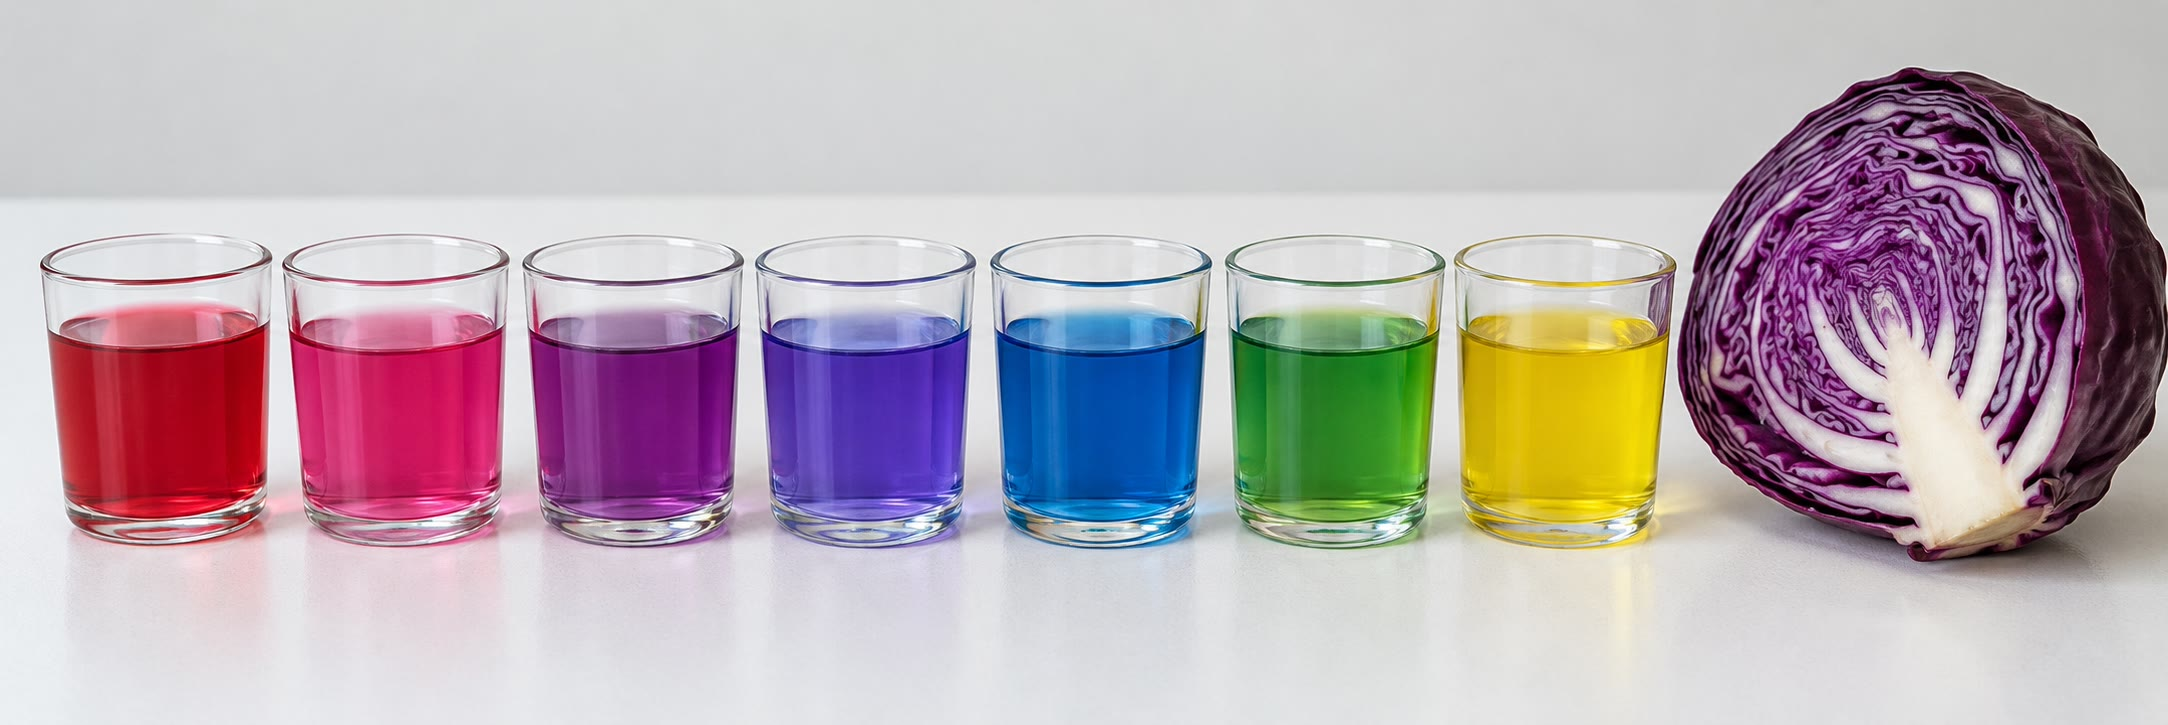
\includegraphics[width=0.55\linewidth]{images/book1/ai/g9-red-cabbage.jpg}

{\small Rodekoolsap, door een docent bereid, verandert van kleur met de
\omterm{def:g9:acids-bases-ph:ph}{pH}: rood in zuren, violet rond neutraal, blauw, groen en dan geel in
steeds basischere oplossingen.}
\end{omfigure}

\section{Veilig omgaan met bijtende producten}

\begin{safety}{\ghs[0.85cm]{GHS05}\ghs[0.85cm]{GHS07}}
% ledger: ghs:HCl, ghs:NaOH
Geconcentreerd zoutzuur en natriumhydroxide (de base van ontstoppers)
dragen het pictogram voor bijtende stoffen, GHS05: ze veroorzaken
ernstige brandwonden aan huid en ogen en tasten metalen aan. GHS07:
irriterend. Veiligheidsbril en handschoenen; een spat wordt meteen met
veel water weggespoeld.
\end{safety}

\begin{remark}[Meng nooit schoonmaakmiddelen]\label{rem:g9:acids-bases-ph:mix}
Zure en basische producten reageren met elkaar, soms heftig, en sommige
\omterm{def:g6:pure-substances-and-mixtures:mixture}{mengsels} geven giftige gassen af: bleekwater gemengd met een zure
ontkalker geeft chloor af. Schoonmaakmiddelen meng je nooit.
\end{remark}

\section{Oefeningen}

\begin{exercise}[$\star$]\label{exo:g9:acids-bases-ph:1}
Zuur, basisch of neutraal? Een oplossing met \omterm{def:g9:acids-bases-ph:ph}{pH} 3, een met \omterm{def:g9:acids-bases-ph:ph}{pH} 7, een met
\omterm{def:g9:acids-bases-ph:ph}{pH} 11.
\end{exercise}

\begin{exercise}[$\star$]\label{exo:g9:acids-bases-ph:2}
Welke \omterm{def:g9:ions:ion}{ionen} zijn er het talrijkst in een \omterm{def:g9:acids-bases-ph:acidic}{zure oplossing}? En in een
basische?
\end{exercise}

\begin{exercise}[$\star$]\label{exo:g9:acids-bases-ph:3}
Zet met de pH-schaal van dit hoofdstuk op volgorde van het meest zuur
tot het meest basisch: koffie, zeewater, limoensap, huishoudammonia,
zuiver water.
\end{exercise}

\begin{exercise}[$\star$]\label{exo:g9:acids-bases-ph:4}
Beschrijf hoe je de \omterm{def:g9:acids-bases-ph:ph}{pH} van een oplossing meet met \omterm{def:g9:acids-bases-ph:ph-paper}{pH-papier}.
\end{exercise}

\begin{exercise}[$\star\star$]\label{exo:g9:acids-bases-ph:5}
Een oplossing met \omterm{def:g9:acids-bases-ph:ph}{pH} 4 wordt tien keer verdund met water. Wat is
ongeveer haar nieuwe \omterm{def:g9:acids-bases-ph:ph}{pH}? En als ze honderd keer verdund wordt?
\end{exercise}

\begin{exercise}[$\star\star$]\label{exo:g9:acids-bases-ph:6}
Kan een \omterm{def:g9:acids-bases-ph:acidic}{zure oplossing} basisch worden door er water bij te doen? Leg
uit.
\end{exercise}

\begin{exercise}[$\star\star$]\label{exo:g9:acids-bases-ph:7}
Waarom moet je een zuur in water gieten, en niet andersom?
\end{exercise}

\begin{exercise}[$\star\star$]\label{exo:g9:acids-bases-ph:8}
Op een fles staat het pictogram GHS05. Wat betekent dat? Noem twee
voorzorgsmaatregelen.
\end{exercise}

\begin{exercise}[$\star\star$]\label{exo:g9:acids-bases-ph:9}
Hoeveel keer moet je een zuur tien keer verdunnen om van \omterm{def:g9:acids-bases-ph:ph}{pH} 1 naar \omterm{def:g9:acids-bases-ph:ph}{pH} 4
te gaan? Hoe groot is de totale verdunning?
\end{exercise}

\begin{exercise}[$\star\star$]\label{exo:g9:acids-bases-ph:10}
Magnesiamelk wordt ingenomen tegen maagzuur. Leg met de pH-schaal uit
waarom.
\end{exercise}

\begin{exercise}[$\star\star\star$]\label{exo:g9:acids-bases-ph:11}
De \omterm{def:g9:acids-bases-ph:ph}{pH} van de oceaan is sinds het industriële tijdperk met ongeveer 0.1
gedaald. Is de oceaan nu zuur? In welke richting verandert hij, en
waarom?
\end{exercise}

\begin{exercise}[$\star\star\star$]\label{exo:g9:acids-bases-ph:12}
Een leerling meet de \omterm{def:g9:acids-bases-ph:ph}{pH} van dezelfde azijn met \omterm{def:g9:acids-bases-ph:ph-paper}{pH-papier} (3) en met een
\omterm{def:g9:acids-bases-ph:ph-paper}{pH-meter} (2.6). Leg uit waarom de twee resultaten verschillen en welk
nauwkeuriger is.
\end{exercise}

\section{Probleem: Gemorst zuur}

\begin{problem}[{Weekendprobleem --- een liter zuur gemorst in een
gootsteen van het laboratorium, en waarom verdunnen niet de oplossing is}]
\label{pb:g9:acids-bases-ph:1}
Een fles met \qty{1}{L} verdund zoutzuur, met \omterm{def:g9:acids-bases-ph:ph}{pH} 2, breekt in een
gootsteen van het laboratorium. In de afvoer mag geen oplossing komen met
een \omterm{def:g9:acids-bases-ph:ph}{pH} onder 5. Gebruik de regel van dit hoofdstuk: voor dit zuur
verhoogt elke tienvoudige verdunning de \omterm{def:g9:acids-bases-ph:ph}{pH} met één eenheid.

\medskip
\noindent\textbf{Deel I --- Het zuur.}
\begin{enumerate}
  \item Is de oplossing zuur, neutraal of basisch? Welke \omterm{def:g9:ions:ion}{ionen} bevat ze
        het meest?
  \item Welk pictogram hoort er op de fles te staan, en waarom?
  \item De docent meet de \omterm{def:g9:acids-bases-ph:ph}{pH} met een \omterm{def:g9:acids-bases-ph:ph-paper}{pH-meter} in plaats van met
        \omterm{def:g9:acids-bases-ph:ph-paper}{pH-papier}. Noem één voordeel.
  \item Hoeveel meer \ce{H+}-ionen zitten er in een liter met \omterm{def:g9:acids-bases-ph:ph}{pH} 2 dan in
        een liter met \omterm{def:g9:acids-bases-ph:ph}{pH} 3 van hetzelfde zuur?
\end{enumerate}

\medskip
\noindent\textbf{Deel II --- Verdunnen.}
\begin{enumerate}[resume]
  \item Hoeveel oplossing krijg je als je de liter zuur tien keer
        verdunt? Wat is de \omterm{def:g9:acids-bases-ph:ph}{pH}?
  \item Hoeveel tienvoudige verdunningen zijn er nodig om \omterm{def:g9:acids-bases-ph:ph}{pH} 5 te
        bereiken?
  \item Hoeveel oplossing zou dat in totaal opleveren?
  \item Zou je de oplossing met genoeg water basisch kunnen maken? Leg
        uit.
\end{enumerate}

\medskip
\noindent\textbf{Deel III --- Een betere manier.}
De docent voegt in plaats daarvan beetje bij beetje een oplossing van een
base toe tot het \omterm{def:g9:acids-bases-ph:ph-paper}{pH-papier} 7 aangeeft: de \ce{H+}-ionen van het zuur
reageren met de \ce{OH-}-ionen van de base.
\begin{enumerate}[resume]
  \item Schrijf de vergelijking op van de reactie tussen \ce{H+}- en
        \ce{OH-}-ionen.
  \item Waarom is dit beter dan verdunnen?
  \item Noem een basisch product uit het dagelijks leven waarmee je in
        een keuken een klein beetje gemorste azijn zou kunnen opruimen.
  \item Bereken hoeveel water je aan de liter zuur zou moeten toevoegen om
        hem op \omterm{def:g9:acids-bases-ph:ph}{pH} 5 te brengen.
\end{enumerate}
\end{problem}
